\documentclass[11pt]{article}

% Common packages
\usepackage{amsmath}
\usepackage{amssymb}
\usepackage{amsthm}
\usepackage{geometry}
\usepackage{enumitem}
\usepackage{graphicx}
\usepackage{titlesec}
\usepackage{tikz}
\usepackage{pgfplots}
\pgfplotsset{compat=1.18}

% Page setup
\geometry{margin=0.5in}
\setlist[itemize]{topsep=2pt,itemsep=2pt,parsep=0pt}

% --- Load hyperref late, then bookmark AFTER hyperref ---
\usepackage[hidelinks]{hyperref}   % load near the end
\usepackage{bookmark}              % must come after hyperref

% Page setup
\geometry{margin=0.5in}
\setlist[itemize]{topsep=2pt,itemsep=2pt,parsep=0pt}

% Short labels
\newcommand{\thm}{\underline{\textbf{Thm.}} }
\newcommand{\defn}{\underline{\textbf{Def.}} }
\newcommand{\prop}{\underline{\textbf{Prop.}} }

% Title info
\title{Econ 4390 Notes - Economics of Education}
\author{Michael Lee}

\begin{document}
\maketitle

\tableofcontents

\newpage

\section{Syllabus / How to Class Works}

\begin{itemize}
    \item Use this email: guillaumevdb@gmail.com. Put Econ 4390 in the SUBJECT
    \item There are no OH. Email Guillaume to figure out when to talk to him about class questions
    \item No HW or participation grade. Grade is the midterm, group project, and final
    \item See syllabus
    \item \textbf{Group Project}
    \begin{itemize}
        \item Groups are 2-4 people
        \item Topic can be on whatever you want BUT we will go over various topics you could present on
        \item All group members will ahve the same grade in the end
        \item These will be toward the end of the semester. 30 min / presentation
        \item Groups will randomly be drawn day of to present. Thus, be ready to present on Day 1
        \item Need to give Guillaume a slide print out BEFORE the presentation begin
    \end{itemize}
    \item Exams should take 20 min
    \item He will frequently leave open problems on the board. These are practice midterm / final questions
    \item The final will contain 1 midterm question
    \item Math will involve power functions and basic derivates. Interpreting the math will give you problems on the exams --- not the maths
    \item Exams are conceptual + math. No MC or TF
\end{itemize}

\section{Intro}
\begin{itemize}
    \item This course will discuss education and what impacts education has on:
    \begin{enumerate}
        \item Macroeconomy
        \item Human experience
        \item Other topics
    \end{enumerate}
    \item This course will cover K-12 and college / university education
    \item \defn Human Capital, (\(h \in \mathbb{R}\)): Input into the production function of any FIRM based on hardskills and softskills a person can RENT to a FIRM
    \item \defn Time worked: \(n \in \mathbb{R}\)
    \item \defn Effective Labor Supply: \(h \cdot n\)
    \item \defn Wage per Effective Unit of Labor per Time Period: \((w)\)
    \item \defn `Wage Rate': \(w \cdot h\)
    \begin{itemize}
        \item \(wh\) together are observable
        \item However, \(w\) and \(h\) independently are not observable
    \end{itemize}
    \item \defn Paycheck: \(w \cdot h \cdot n\)
\end{itemize}

\section{Model 1 - Why are more people going to college?}
\begin{itemize}
    \item Suppose ``life" last for 2 periods
    \item Period 1:
    \begin{itemize}
        \item Time in college
        \item Tuition, \(e > 0 - \text{``opportunity cost of college"}\)
    \end{itemize}
    \item Period 2:
    \begin{itemize}
        \item Time after the college
    \end{itemize}
    \item People who attend college don't work in Period 1 and work in Period 2
    \item People who do NOT college college work in Period 1 and Period 2
    \item People differ in their ability, \(a > 0\). \(a\) is given at the start of Period 1
    \item Assume there are perfect credit markets (you can borrow and lend AS MUCH AS YOU WANT)
    \item Income for non-college people, \(I_{HS} = w \cdot a\)
    \item Income for college grads, \(I_{C} = w \cdot h \cdot a\)
\end{itemize}

\begin{itemize}
    \item Wealth vs. Income
    \begin{itemize}
        \item Income, \(I\), is how much you get paid (typically)
        \[
        I = \text{Price of skills} \times \text{Quantity of skills}
        \]
        \item Wealth is the total remaining amount of Income accrued
        \item The value of wealth decreases over time due to inflation
        \item \defn Interest rate (\(r\)) - The amount you would pay today to get a dollar tomorrow
        \item Hence, the present value of a dollar is
        \[
            \frac{1}{1+r}
        \]
        \item Suppose I invest \(\frac{1}{1+r}\)
        \[
            \frac{1}{1+r} \cdot (1+r) = 1
        \]
    \end{itemize}
    \item Suppose Income in Period \(i\) is \(y_i\)
    \item Thus, the present value of Income is 
    \[
        y_1 + \frac{y_2}{1+r}
    \]
    \item Hence, for HS grads, the present value of Income is:
    \[
        W_0(a) = aw + \frac{aw}{1+r}
    \]
    \item And, for college grads, the present value of Income is:
    \[
        W_1(a) = -e + \frac{ahw}{1+r}
    \]
    \item Graphing this: \\
    
    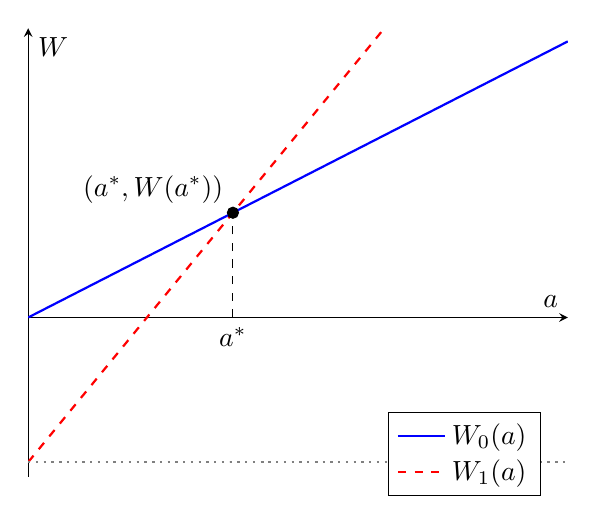
\begin{tikzpicture}
        \begin{axis}[
          axis lines=middle,
          xlabel={$a$},
          ylabel={$W$},
          xmin=0, xmax=10,
          ymin=-110, ymax=200,
          domain=0:10,
          samples=100,
          legend style={at={(0.95,0.05)},anchor=east},
          xtick=\empty, ytick=\empty   % <-- remove ticks
        ]
      
        % Parameters
        \def\w{10}
        \def\h{5}
        \def\r{0.1}
        \def\e{100}
      
        % W0(a) = a w + (a w)/(1+r)
        \addplot[blue, thick] {x*\w + (x*\w)/(1+\r)};
        \addlegendentry{$W_0(a)$}
      
        % W1(a) = -e + (a h w)/(1+r)
        \addplot[red, thick, dashed] {- \e + (x*\h*\w)/(1+\r)};
        \addlegendentry{$W_1(a)$}
      
        % Horizontal line at -e
        \addplot[dotted, gray, thick, domain=0:10] {- \e};
        \node[anchor=west] at (axis cs:10,-100) {$-e$};
      
        % Intersection point a*
        \pgfmathsetmacro{\astar}{- \e / (\w + \w/(1+\r) - (\h*\w)/(1+\r))}
        \addplot[mark=*,black]
          coordinates {(\astar,{(\astar*\w + (\astar*\w)/(1+\r))})};
        \node[above left]
          at (axis cs:\astar,{(\astar*\w + (\astar*\w)/(1+\r))})
          {$(a^*,W(a^*))$};
      
        % Projection down to x-axis
        \draw[dashed]
          (axis cs:\astar,0) -- (axis cs:\astar,{(\astar*\w + (\astar*\w)/(1+\r))});
        \node[below] at (axis cs:\astar,0) {$a^*$};
      
        \end{axis}
      \end{tikzpicture}      
      
    \item Here, \(a^*\) is \(a\) s.t. \(W_0 = W_1\)
    \begin{itemize}
        \item If your \(a = a^*\), you are indifferent financially going to college
        \item If your \(a > a^*\), you are better off financially going to college
        \item If your \(a < a^*\), you are worse off financially going to college
    \end{itemize}
    \item Are we certain \(\exists (a^* > 0)\)?
    \item Yes \(\iff\) \(W_1(a)\) is steeper than \(W_0(a)\)
    \[
        \frac{dW_0(a)}{da} = w + \frac{w}{1+r}
        \quad \text{and} \quad 
        \frac{dW_1(a)}{da} = \frac{wh}{1+r}
    \]
    \[
        \frac{dW_1(a)}{da} = \frac{wh}{1+r} > \frac{dW_0(a)}{da} = w + \frac{w}{1+r}
        \Rightarrow
        h-1 > 1+r
    \]
    \item Hence, our condition is
    \[
        \frac{wh}{1+r} > w + \frac{w}{1+r}
        \iff
        h-1 > 1+r
    \]
    \item What is \(a^*\)?
    \begin{itemize}
        \item \(a^*\) is defined as some \(a\) s.t. \(W_0(a^*) = W_1(a^*)\)
        \[
            W_0(a^*) = a^*w + \frac{a^*w}{1+r} =  W_1(a^*) = -e + \frac{a^*wh}{1+r}
        \]
        \[
            a^*w + \frac{a^*w}{1+r} - \frac{a^*wh}{1+r}
            = a^*w \left( 1 + \frac{1}{1+r} - \frac{h}{1+r} \right)
            = -e
        \]
        \[
            a^*w \left( \frac{1+r+1-h}{1+r} \right)
            = a^*w \left( \frac{(h-1) - (r+1)}{1+r} \right)
            = -e
        \]
        \[
            a^*
            = \frac{e}{w} \cdot \frac{1+r}{(h-1) - (r+1)}
        \]
    \item Using this equation, we notice the following statics:
    \begin{itemize}
        \item \(e\) and \(r\) are \textbf{directly proportional} to \(a^*\). Equivalently, \(\frac{da^*}{dw}, \frac{da^*}{dh} < 0\)
        \item \(w\) and \(h\) are \textbf{inversely proportional} to \(a^*\). Equivalently, \(\frac{da^*}{de}, \frac{da^*}{dr} > 0\)
    \end{itemize}
    \item So what are the key drivers right now?
    \end{itemize}
    \item So what is the rate of return on this investment?
    \begin{itemize}
        \item \defn Rate of return:
        \[
            \frac{\text{``what it pays''} - \text{``what it costs''}}{\text{``what it costs''}}
        \]
        \item College pays: \(awh-aw\) (because \(aw\) is guaranteed to all HS grads)
        \item College costs: \(e+aw\)
        \item Let the rate of return be \(\rho(a)\)
        \[
            \rho(a) = 
            \frac{
                aw(h-1) - (e+aw)
            }
            {
                e+aw
            }
        \]
        \item Thus,
        \[
            \rho(a) = 
            \frac{
                aw(h-1) - (e+aw)
            }
            {
                e+aw
            }
            =
            \frac{aw(h-1)}{e+aw} - \frac{e+aw}{e+aw}
            = 
            \frac{aw(h-1)}{e+aw} - 1
        \]
        \[
            \Rightarrow
            1 + \rho(a)
            = \frac{h-1}{1+ \frac{e}{aw}}
            = \frac{aw(h-1)}{aw+e}
        \]
        \item Recall:
        \[
            a^*
            = \frac{e}{w} \cdot \frac{1+r}{(h-1) - (r+1)}
        \]
        \item Hence,
    \end{itemize}
    \[
        1 + \rho(a^*)
        = \frac{h-1}{1+ \frac{e}{a^*w}}
        = \frac{h-1}{1+ \frac{e}{\frac{e}{w} \cdot \frac{1+r}{(h-1) - (r+1)}w}}
        = \frac{h-1}{1+ \frac{e}{e \cdot \frac{1+r}{(h-1) - (r+1)}}}
        = \frac{h-1}{1+ \frac{(h-1) - (r+1)}{1+r}}
    \]
    \[
        = \frac{(h-1)(1+r)}{(1+r)+ (h-1) - (r+1)}
        = 1 + r 
        \Rightarrow \rho(a^*) = r
    \]
    \item Conceptually, this means that \textbf{rate of return} on education for people whose ability, \(a\), makes them indifferent to going to college or not going to college have an ability equal to the interest rate, \(r\).
    \item \(\forall a > a^*\), \textbf{rate of return} on education be better than the interest rate (so it's a good investment)
    \item \(\forall a < a^*\), \textbf{rate of return} on education be worse than the interest rate (so it's a bad investment)
    \item Now, we will interpret \(h-1 > 1+r\)
    \begin{itemize}
        \item Recall 
        \[
            1 + \rho(a^*)
            = \frac{h-1}{1+ \frac{e}{a^*w}}
        \]
        \item Thus,
        \[
            \lim_{a \rightarrow \infty} (1 + \rho(a))
            = 
            h-1
            > 1 - r
        \]
        \item The interpretation is that for individuals with exceptional ability, their rate of return is ALWAYS better than the interest rate (so it's a worthwhile investment)
    \end{itemize}
    \item \textbf{Practice Drills}
    \begin{enumerate}
        \item In Excel, create a graph where you fix \(e,h,r\), have a \(w_{min}, w_{max}\) and graph a function showing \(f:w \rightarrow a^*\). Play around with the graph and think about conceptually WHY changing the input variables impacts \(a^*\)
    \end{enumerate}
    \item How do we incorporate family wealth into the model?
    \begin{itemize}
        \item For this model, we will assume your family transfer some amount of wealth, \(A \in \mathbb{R}\) after high school
        \[
            W_0(a) = wa + \frac{aw}{1+r} + A
            \quad \text{and} \quad
            W_1(a) = -e + \frac{awh}{1+r} + A
        \]
        \item If we make \(A\) conditional \(a\), this implies that ability is a trait that is carried from generation to generation. Therefore, people with higher wealth and likely to have high ability and vice versa
        \item This could be because of \(\dots\)
        \begin{enumerate}
            \item Richer parents can give their kids more resources, leading to a higher \(a\)
            \item Parents with high ability create high ability kids (because genetics and/or culture)
        \end{enumerate}
        \[
            W_0(a) = wa + \frac{aw}{1+r} + A(a)
            \quad \text{and} \quad
            W_1(a) = -e + \frac{awh}{1+r} + A(a)
        \]
        \item \(A\) has no impact on \(a^*\), \(\rho(a)\), or \(\frac{dW_0(a)}{da} > \frac{dW_1(a)}{da}\)
    \end{itemize}
    \item Credit Constraints
    \begin{itemize}
        \item \defn Early Credit Constraint - Capability to investment in a child's education before college. Impacts a student's ability (\(a\)) to attend college
        \item \defn Late Credit Constraint - Capability to investment in a child's education in college
        \item Early credit constraint is much more important in determining college attainment than late credit constraints (according to the literature). This is why people pay so much for good preschool and elementary school
        \item \textbf{This relationship could be a good presentation topic}
    \end{itemize}
\end{itemize}

\newpage

\section{Deterministic Wage Growth}
\begin{itemize}
    \item \defn Deterministic - Something is impacted in a determinable, non-random way
    \item \defn Stochastic - Something is impacted in an indeterminable, randomy way
    \item Thus, a \textbf{Deterministic Wage Growth model} shows how wages grow in a determinable, non-random way
    \item Suppose wages, \(w\), increase a a constant rate, \(g\):
    \[
        w_{t+1} = (1+g)w_t
        \Rightarrow
        w_{t} = (1+g)w_{t-1} = (1+g)^tw_0
        \Rightarrow
        \ln(w_t)
        = \ln \big( (1+g)^tw_0 \big)
        = t \cdot \ln(1+g) + \ln(w_0)
    \] 
    \item Thus,
    \[
        \frac{d \ln(w_t)}{dt} = \ln(1+g)
    \]
    \item And so, the log-wage is a straight line (over time). We will assume that \(w\) increases in a step-wise manner
    \item Factoring this into our previous wealth model,
    \[
        W_0(a) = wa + \frac{aw(1+g)}{1+r}
        \quad \text{and} \quad
        W_1(a) = -e + \frac{awh(1+g)}{1+r}
    \]
    \item Now, let's find \(a^*\) (\textbf{Good practice drill to do at home!!})
    \[
        W_0(a^*) = wa + \frac{a^*w(1+g)}{1+r} = W_1(a^*) = -e + \frac{a^*wh(1+g)}{1+r}
        \Rightarrow
        \boxed{a^* = \frac{e}{w} \cdot \frac{1+r}{(h-1)(1+g) - (1+r)}}
    \]
    \item Hence, \(g\) and \(a^*\) are \textbf{inversely proportional}
    \item Now we will look at the rate of return and see if \(\rho(a^*) = r\)
    \begin{itemize}
        \item College pays: \(awh(1+g) - aw(1+g) = aw(1+g)(h-1)\)
        \item College costs: \(e + aw\)
        \item Hence,
        \[
            1 + \rho(a)
            = \frac{(1+g)aw(h-1) - (e+aw)}{e+aw}
            = \frac{(1+g)(h-1)}{1 + \frac{e}{aw}}
        \]
        \item Now we plug in \(a^*\)
        \[
            1 + \rho(a^*)
            = \frac{(1+g)(h-1)}{1 + \frac{e}{a^*w}}
            = \frac{(1+g)(h-1)}{1 + \frac{e}{\frac{e}{w} \cdot \frac{1+r}{(h-1)(1+g) - (1+r)} \cdot w}}
            = \frac{(1+g)(h-1)}{1 + \frac{(h-1)(1+g) - (1+r)}{1+r}}
            = \frac{(1+g)(h-1)}{1 + \frac{(h-1)(1+g)}{1+r} - 1}
        \]
        \[
            1 + \rho(a^*)
            = \frac{(1+g)(h-1)}{\frac{(h-1)(1+g)}{1+r}}
            = 1 + r
        \]
        \item Thus,
        \[
        \rho(a^*) = r
        \]
        \item The lesson here is that we made things closer to reality, but it did not lead to much additional insight
        \item More complicated model \(\nRightarrow\) More insightful model
    \end{itemize}

\end{itemize}

\newpage

\section{Stochastic Wage Growth}
\subsection*{Defining Random Variables}
\begin{itemize}
    \item Suppose \(X\) is a random variable that can take value \(x_i\) with probability \(p_i\) \((i \in [n] \subseteq \mathbb{N})\)
    \item All \(x_i\) are possible realizations of \(x\), so \(\sum_{i} p_i = 1\)
    \item Recall \(E(X) = \sum_{i} x_i \cdot p_i\)
    \item \(E\) is linear. In other words:
    \[
        E(\alpha X + \beta) = \sum_{i} p_i(\alpha x_i + \beta) = \alpha \cdot E(X) + \beta
        \quad (\alpha, \beta \in \mathbb{R})
    \]
\end{itemize}

\subsection*{Going into the model . . .}
\begin{itemize}
    \item Suppose a wage rate in the second period, \(w'\) is not known in Period 1. Thus, in Period 1:
    \[
        W_0(a)
        = E \left( aw + \frac{aw'}{1+r} \right)
        \quad \text{and} \quad
        W_1(a)
        = E \left( -e + \frac{ahw'}{1+r} \right)
    \]
    \item which is equivalent to . . .
    \[
        W_0(a)
        = aw + \frac{aE(w')}{1+r}
        \quad \text{and} \quad
        W_1(a)
        = -e + \frac{ahE(w')}{1+r}
    \]
    \item Hence, if \(W_0(a^*) = W_1(a^*)\)
    \[
        W_0(a^*)
        = a^*w + \frac{a^*E(w')}{1+r}
        = W_1(a^*)
        = -e + \frac{a^*hE(w')}{1+r}
    \]
    \[
        -e
        = a^*w \left( 1 + \frac{E(w')/w - hE(w')/w}{1+r} \right)
        = a^*w \left( \frac{(1+r) + E(w')/w - hE(w')/w}{1+r} \right)
    \]
    \[
        \boxed{a^*
        = \frac{-e}{w} \cdot \frac{1+r}{(h-1)E(w')/w - (1+r)}}
    \] 
    \item Recall the solution for the \textbf{Deterministic Wage Growth} model
    \[
        a^* = \frac{e}{w} \cdot \frac{1+r}{(h-1)(1+g) - (1+r)}
    \]
    \item Thus, if \(\frac{E(w')}{w} = 1+g\), we can expect \(a^*\) to be the same in deterministic and stochastic models
    \item If \(E(w') = w\), we expect no growth and so \(a^*\) is the same as in the basic model
\end{itemize}

\subsection*{Utility Functions}
\begin{itemize}
    \item Recall utility function \(U: \mathbb{R}^n \rightarrow \mathbb{R}, c \rightarrow r\)
    \item Typicaly, we think of utility as continuous. Imagine it's discrete:
    \item Suppose that consumption, \(c_i\) occurs with probability \(p_i\) \((i \in [n])\)
    \item Thus, the expected utility of consumption is:
    \[
        E(U(c)) = \sum_i p_i \cdot U(c_i)
    \]
    \item However, the utility of expected consumption is:
    \[
        U(E(c)) = U\left( \sum_i p_i \cdot c_i \right)
    \]
    \item When \(U(c)\) is monotonic and \(\forall c\), \(U''(c) < 0\),
    \[
        U(E(c)) > E(U(c))
    \]
    \item This proves the utility from the expected consumption is better than the expected value of the utility given discrete consumption options
\end{itemize}

\section{Work in College}
\begin{itemize}
    \item Suppose people work a fraction of their time, \(1 - \theta\) in college (\(\theta \in [0,1]\))
    \item Hence, our value functions become:
    \[
        W_0(a)
        = aw + \frac{aw}{1+r}
        \quad \text{and} \quad
        W_1(a)
        = -e + aw(1 - \theta) + \frac{ahw}{1+r}
    \]
    \item Which is not super true as the more time you spend on working in college, the less time you spend studying. Thus, \(h\) is conditional on \(\theta\)
    \item Hence, your goal should be:
    \[
        W_1(a)
        = \max_{\theta} \left\{ -e + aw(1 - \theta) + \frac{ah(\theta)w}{1+r} \right\}
    \]
    \item \textbf{Practice Drills}:
    \begin{itemize}
        \item \textbf{Prove:} \(\rho(a) = \frac{aw(h-1) - (e + aw \theta)}{e + aw\theta}\)
        \item \textbf{Prove:} \(a^* = \frac{e}{w} \cdot \frac{1+r}{(h-1) - (1+r)\theta}\)
        \item \textbf{Prove:} For \(\theta\) that maximizes \(W_1(a) = \max_{\theta} \left\{ -e + aw(1 - \theta) + \frac{ah(\theta)w}{1+r} \right\}\) is independent of \(a\)
        \[
            W_1
            \quad \Rightarrow \quad
            \frac{\partial W_1}{\partial \theta}
            = -aw + \frac{aw}{1+r} h'(\theta)
            = aw \left( \frac{h'(\theta)}{1+r} - 1 \right)
            = 0
        \]
        \[
        \frac{h'(\theta)}{1+r} - 1 = 0
        \quad \Rightarrow \quad
        h'(\theta) = 1 + r
        \quad \Rightarrow \quad
        \theta = h^{-1}(1+r)
        \]
        \[
            \square
        \]
        \item \textbf{Prove:} For a monotonic function \(U(c)\) where \(\forall c_2 > c_1\), \(U'(c_1) > U'(c_2)\) and \(P(c_i) = p_i\), prove \(U(E(c)) > E(U(c))\)
    \end{itemize}
    \item We will assume that \(h(\theta)\) in an increasing, monotonic function and first-order derivitable. We call the change in \(\theta\) and \(h(\theta)\) the \textbf{marginal productivity}
    \item Let's find \(\theta\) that maximizes \(W_1\)
    \[
        W_1
        \quad \Rightarrow \quad
        \frac{\partial{W_1}}{\partial \theta}
        = 0 = -aw + \frac{awh'(\theta)}{1+r}
    \]  
    \[
        \Rightarrow \quad aw = \frac{awh'(\theta)}{1+r}
    \]
    \begin{itemize}
        \item We can think of \(aw\) as the opportunity cost of working one more hour and \(\frac{awh'(\theta)}{1+r}\) as the opportunity benefit of working one more hour.
        \item If \(aw \neq \frac{awh'(\theta)}{1+r}\) (i.e. \(aw > \frac{awh'(\theta)}{1+r}\) or \(aw < \frac{awh'(\theta)}{1+r}\)), we are not at the optimum. Thus we can spend less or more time working to reach an optimum, respectively
        \item Going back to the maths,
    \end{itemize}
    \[
        h'^{-1}\!(\theta) = 1+r
        \quad \Rightarrow \quad
        \theta = h'^{-1}\!(1+r)
    \]
    \begin{itemize}
        \item In plain English, if \(a\) has no impact on \(\theta\), this is because 
    \end{itemize}
    \item Consider the following function:
    \[
        W_1(a)
        = \max_\theta \left\{ -e + aw(1-\theta) + \frac{awh(a \theta) w}{1+r} \right\}
    \]
    \item Thus,
    \[
        \frac{\partial W_1}{\partial \theta} = 0 = - aw + \frac{a^2wh'(a \theta)}{1+r}
        \quad \Rightarrow \quad
        aw = \frac{a^2wh'(a \theta)}{1+r}
        \quad \Rightarrow \quad
        1 = \frac{a h'(a \theta)}{1+r}
        \quad \Rightarrow \quad
        1+r = a h'(a \theta)
    \]
    \[
        \Rightarrow \quad
        \frac{1+r}{a} = h'(a\theta)
        \quad \Rightarrow \quad
        h'^{-1}\!\left( \tfrac{1+r}{a} \right) = a\theta
        \quad \Rightarrow \quad
        \theta = \frac{h'^{-1}\!\left( \tfrac{1+r}{a} \right)}{a}
    \]

\end{itemize}

\newpage

\section{The College Premium}
\begin{itemize}
    \item We notice that wages for workers aged 30-60 is pretty constant over time.
    \item However, college educated workers have gone from making \(30\%\) more than non-college educated workers to \(80\%\).
    \item Literature suggests this is because of the IT revolution (starting in the 1980s).
    \item Recall \(W_0\), \(W_1\), and \(a^*\)
    \item The college premium, \(CP\), is defined as:
    \[
        CP = \frac{\text{Earnings of the average college-educated worker}}{\text{Earnings of the average non-college-educated worker}}
    \]
    \item Thus, in our model,
    \[
        CP
        = \frac{E(ahw|a>a^*)}{E(aw|a<a^*)}
        = \frac{wh \cdot E(a|a>a^*)}{w \cdot E(a|a<a^*)}
        = h \times \frac{E(a|a>a^*)}{E(a|a<a^*)}
    \]
    \item Note that \(h\) is what makes \(CP\) specific to an individual
    \item \defn Selection Effect: \(\frac{E(a|a>a^*)}{E(a|a<a^*)}\)
    \item Recall \(W_0\) and \(W_1\). We can find the \textbf{Lifetime College Premium}
\end{itemize}
\[
    CP
    = \frac{W_1}{W_0}
    = \frac{\frac{E(awh | a > a^*)}{1+r}}{E(aw + \frac{aw}{1+r} | a < a^*)}
    = \frac{\frac{wh}{1+r} \cdot E(a|a > a^*)}{w\left(1 + \frac{1}{1+r}\right) \cdot E(a | a < a^*)}
    = \frac{h}{2+r} \cdot \frac{E(a | a > a^*)}{E(a | a < a^*)}
\]
\begin{itemize}
    \item Let the density of ability be \(f(a)\). Also, let \(a \in [a_m, a_M]\) Note that:
    \[
        p(a) = \int_{a_m}^{a} f(a) \, da
    \]
    \item Suppose \(f(a) \sim U(a_m, a_M)\). Thus,
    \[
        E(a) = \frac{a_m + a_M}{2};
        \quad
        E(a | a > a^*) = \frac{a^* + a_M}{2};
        \quad
        E(a | a < a^*) = \frac{a^* + a_m}{2}
    \]
    \item As a side note,
    \[
        1 = \int_{a_m}^{a_M} f(a) \, da \quad \Rightarrow \quad \forall a, \, f(a) = \frac{1}{a_M - a_m}
    \]
    \item This impacts \(CP\)
    \[
        CP
        = \frac{E(a | a > a^*)}{E(a | a < a^*)}
        = \frac{\frac{a^* + a_M}{2}}{\frac{a^* + a_m}{2}}
        = \frac{a^* + a_M}{a^* + a_m}
    \]
    \[
        \frac{\partial}{\partial a^*}\left(\frac{a^* + a_M}{a^* + a_m}\right)
        = \frac{a_m - a_M}{(a^* + a_m)2}
        < 0
    \]
\end{itemize}
\newpage

\section{Skill-based Technology}
\begin{itemize}
    \item Starting in the 1980s, college educated people began earning way more and by 2000 earned more than non-college educated individuals. We suspect this is due to the IT revolution. We will create a series of models explainin this effect.
    \item Let our production, \(Y = F(K, L)\), be conditional on labor, \(L\), and capital, \(K\).
    \item Note that \(F(0, L) = F(K, 0) = 0\) and \(\forall L, K \neq 0, \, F(K, L)\geq 0\). Also, marginal products are decreasing.
    \item \defn Marginal returns: How much does output change when one input changes a little
    \item \defn Retursn to scale: How much does output change when all inputs change in the same proportionally (i.e. \(F(\lambda K, \lambda L)\) where \(\lambda \in \mathbb{R}\))
    \item \defn Constant returns to scale (CRS): If all inputs are multiplied by \(\lambda \in \mathbb{R}\), the output is multiplied by \(\lambda\) (i.e. \(\lambda F(K, L) = F(\lambda K, \lambda L)\))
    \begin{itemize}
        \item NOTE: CRS implies that 1 firm of size \(k\) produces as much as \(k\) firms of size 1.
    \end{itemize}
    \item \textbf{Practice Drills:} Prove/disprove the following functions show CRS
    \begin{itemize}
        \item Linear: \(F(K, L) = aK + bL\)
        \item Cobb-Douglas: \(F(K, L) = K^\alpha \cdot L ^{1 - \alpha}\)
        \item Constant Elasticity Substitution (CES): \(F(K, L) = (K^\alpha + L^\alpha)^{1/\alpha}\)
    \end{itemize}
    \item Define the following marginal product of labor and capital (respectively):
    \[
        MP_L = \frac{\partial Y}{\partial L};
        \quad
        MP_K = \frac{\partial Y}{\partial K}
    \]
    \item Firms care about maximization profit, \(\pi\).
    \item Let \(r\) be the price at which capital is hired
    \item Let the \textbf{real wage}, \(w\), be the price at which labor is hired
    \item We will assume that all goods produced are sold
    \[
        \pi = F(K, L) - (rK + wL)
    \]
    \item This model assumes the firm has no power over choosing \(r\) or \(w\)
    \item The firm's goal, profit maximization, is:
    \[
        \max_{K, L} \{\pi(K, L)\}
    \]
    \item If \(MP_L > w\), hiring raises profit but lowers \(MP_L\)
    \item If \(MP_L < w\), firing raises profit but raises \(MP_L\)
    \item At optimum, \(MP_L = w\).
    \item Firms hire both high school and college educated workers
    \item Firms hire both types and technology is:
    \[
        Y = F(K, L) \quad \text{where} \quad L=H(L_0,L_1)
    \]
    \item Some notes:
    \begin{itemize}
        \item \(L\) aggregates the total labor supplied by both types of workers
        \item \(H\) is the aggregator for the two types of workers
        \[
            L_0 = \int_{a_m}^{a^*} a \cdot f(a) \, da
            \quad \text{and} \quad
            L_1 = \int_{a^*}^{a_M} a \cdot f(a) \, da
        \]
    \end{itemize}
    \item The firm's maximizaton problem is:
    \[
        \max_{K, L_0, L_1} \{F(K, H(L_0, L_1)) - rK - wL_0 - w_1L_1\}
    \]
    \item and it requires that:
    \[
        w_0 = F_L(K, H(L_0, L_1)) \cdot H_{L_0}(L_0, L_1)
    \]
    \[
        w_1 = F_L(K, H(L_0, L_1)) \cdot H_{L_1}(L_0, L_1)
    \]
    \item Note that:
    \[
        \frac{w_1}{w_0}
        = \frac{H_{L_1}(L_0, L_1)F_L(K, H(L_0, L_1))}{H_{L_0}(L_0, L_1)F_L(K, H(L_0, L_1))}
        = \frac{H_{L_1}(L_0, L_1)}{H_{L_0}(L_0, L_1)}
    \]
    \item This equation implies the marginal return, \(MP\), to each type of workers
    \item Since \(1 = \frac{w_1}{w_0}\),
    \[
        1 = \frac{w_1}{w_0} = \frac{H_{L_0} (L_0, L_1)}{H_{L_1} (L_0, L_1)} \quad \Rightarrow \quad H_{L_1} (L_0, L_1) = H_{L_0} (L_0, L_1)
    \]
    \rule[7pt]{\linewidth}{0.4pt}
    \item \textbf{Practice Drill:} Maximize the firm's output given these functions:
    \[
        F(K, L) = K^{1/3} \cdot L^{2/3}
        \quad \text{and} \quad
        L = H(L_0, L_1) = 5L_0 + L_1
    \]
    \[
        \Rightarrow \quad F_L(K, L) \cdot H_{L_0}(L_0, L_1)
        = F_L(K, L) \cdot 5
        = \frac{10}{3} \left( \frac{K}{L} \right)^{1/3}
    \]
    \item For \(K, L = 10\), \(Y = F(10, 10) = 10\) and \(F_L(10, 10)H_{L_0}(10, 10) = 10/3 = MP_{L_0}\).
    \item Suppose \(w_0, w_1,  r = 1\). Thus,
    \[
        \pi = 10 - 10(1) - 1(1) - 1(5) = -6
    \]
    \item \textbf{Practice Drill:} Claim, if I have \(F(K, L)\) that is CRS, \(F_L\) is a function of \(K/L\) and \(F_K\) is a function of \(K/L\)
    \rule[7pt]{\linewidth}{0.4pt}
    \item Suppose \(w_0 \neq w_1\). Thus,
    \[
        W_0(a) = aw_0 + \frac{aw_0}{1+r}
        \quad \text{and} \quad
        W_1(a) = -e + \frac{ahw_1}{1+r}
    \]
    \item Recall the marginal individual is defined as a person with ability \(a^*\).
    \[
        W_0(a^*) = a^*w_0 + \frac{a^*w_0}{1+r} = W_1(a^*) = -e + \frac{a^*h w_1}{1+r}
    \]
    \[
        a^*w_0 \left( 1 + \frac{1}{1+r} - \frac{h w_1}{w_0 (1+r)} \right) = -e
    \]
    \[
        a^* = \frac{e}{w_0} \cdot \frac{1+r}{(hw_1 / w_0 - 1) - (1+r)}
    \]
    \item Suppose \(H(L_0, L_1) = L_0 + z \cdot L_1\) for some \(z \in \mathbb{R}\). Thus,
    \[
        \frac{w_1}{w_0} = z
        \quad \text{and} \quad
        a^* = \frac{e}{w_0} \cdot \frac{1+r}{(hz-1) + (1+r)}
        \quad \text{and} \quad
        CP = h \cdot z \cdot \frac{E(a | a > a^*)}{E(a | a < a^*)}
    \]
\end{itemize}

\newpage

\section{Multi-period Model}
\begin{itemize}
    \item Suppose that life contained \(T\)-periods, where \(s\)-periods are spent in college. Our model would be:
    \[
        W_0
        = \sum_{i=1}^{T} aw \cdot \left( \frac{1+g}{1+r} \right)^{i-1}
        = aw \cdot \sum_{i=1}^{T} \left( \frac{1+g}{1+r} \right)^{i-1}
    \]
    \[
        W_s
        = -e + \sum_{i = s+1}^{T} awh \cdot \left( \frac{1+g}{1+r} \right)^{i-1}
        = -e + \cdot awh \cdot \sum_{i = s+1}^{T} \left( \frac{1+g}{1+r} \right)^{i-1}
    \]
    \item Note that we typically view \(T\) as the ``life expectancy'' of a person. Here, life expectancy is the number of years a person has left to live.
    \item Where \(W_s\) is the model for the college-educated people spending \(s\)-periods in college.
    \item Note that \(W_s\) is similar to \(W_0\), but they start earning in period \(s+1\). This is because they spent \(s\)-periods in college.
    \item Define the following:
    \[
        D_0 = \sum_{i=1}^{T} \left( \frac{1+g}{1+r} \right)^{i-1}
        \quad \text{and} \quad
        D_s = \sum_{i = s+1}^{T} \left( \frac{1+g}{1+r} \right)^{i-1}
    \]
    \item Thus,
    \[
        W_0 = aw \cdot D_0
        \quad \text{and} \quad
        W_s = -e + awh \cdot D_s
    \]
    \item Solving for \(a^*\) yields:
    \[
        a^* = \frac{e}{w} \cdot \frac{1}{hD_s - D_0}
    \]
    \item \textbf{Practice Drill:} Prove that \(a^* = \frac{e}{w} \cdot \frac{1}{hD_s - D_0}\). Expect for this to be on an exam.
    \item Recall that:
    \[
        \sum_{i=1}^T x^i = \frac{1-x^{T+1}}{1-x}
    \]
    \item Thus, for \(D_0\) and \(D_s\), we have:
    \[
        D_0 = \frac{1- \left( \frac{1+g}{1+r} \right)^{T}}{1- \frac{1+g}{1+r}}
        \quad \text{and} \quad
        D_s = \frac{\left(\frac{1+g}{1+r}\right)^s - \left(\frac{1+g}{1+r} \right)^{T}}{1- \frac{1+g}{1+r}}
    \]
    \item Hence, looking at \(hD_s - D_0\), we have:
    \[
        hD_s - D_0
        = h \cdot \frac{\left(\frac{1+g}{1+r}\right)^s - \left(\frac{1+g}{1+r} \right)^{T}}{1- \frac{1+g}{1+r}} - \frac{1- \left( \frac{1+g}{1+r} \right)^{T}}{1- \frac{1+g}{1+r}}
        = \frac{h\left( \frac{1+g}{1+r} \right)^s - 1 - (h-1)\left( \frac{1+g}{1+r} \right)^{T}}{1- \frac{1+g}{1+r}}
    \]
    \item Note that \(g < r \Rightarrow hD_s - D_0\) is increasing with \(T\), so \(a^*\) is increasing.
    \item If \(g < r\), then educational attainment is increasing with life expectancy.
\end{itemize}

\newpage

\section{Labor Supply}
\begin{itemize}
    \item We notice that people are working less per week over time (1820: 72 hr/wk; 2000: 40 hr/wk).
    \item People also work fewer weeks per year and fewer days per week.x
    \item We also notice that people spend more time in school over time (1870: 7 yr; 1980: 14 yr).
    \item We will assume people care about consumption and leisure time. We will assume that more is better for both.
    \item There are infinitely many indifference curves displaying difference consumption and leisure curve allocations.
\end{itemize}

\[
\begin{tikzpicture}[scale=1.0]
    % Axes (square domain)
    \draw[->] (0,0) -- (7.5,0) node[below right]{Leisure $L$};
    \draw[->] (0,0) -- (0,7.5) node[above left]{Consumption $C$};
  
    % Clip to [0,7]x[0,7]
    \begin{scope}
      \clip (0,0) rectangle (7,7);
  
      % Symmetric indifference curves: C = k / L
      % choose k values that look balanced in the square
      \draw[thick, domain=0.5:7, samples=200] plot (\x,{5/(\x)}) node[pos=0.85, above] {$U_1$};
      \draw[thick, domain=0.5:7, samples=200] plot (\x,{8/(\x)}) node[pos=0.65, above] {$U_2$};
    \end{scope}
  
    % Higher utility arrow
    \draw[->, thick] (4.2,4.2) -- (5.4,5.4) node[above right] {More preferred};
  
    % Axis ticks
    \foreach \x in {1,2,...,7} \draw (\x,0) -- (\x,-0.07) node[below] {\small \x};
    \foreach \y in {1,2,...,7} \draw (0,\y) -- (-0.07,\y) node[left] {\small \y};
\end{tikzpicture}
\]
\begin{itemize}
    \item The rate at which someone with substitute consumption and leisure is the marginal rate of substitution (MRS).
    \item MRS is the slope of the indifference curve.
    \item Let \(c\) be consumption at price \(p\), \(l\) be leisure hours, and \(\omega\) be the wage rate.
    \item Assume there are \(24 \cdot 7 = 168\) hours in a week
    \item The labor supply is \(168 - l\)
    \item This yields the budget curve:
    \[
        p \cdot c = \omega(168 - l)
        \quad \iff \quad
        c = \frac{\omega}{p} (168 - l)
    \]
    \item If \(w = \frac{\omega}{p}\) is the real wage rate and we normalize \(l\) to represent the fraction of the week spent working,
    \[
        c = w(1 - l)
        \quad \iff \quad
        c + wl = w
    \]
    \item Trivially, this budget is a straight line.
    \item The `optimum' is where there are no more preferable points
    \item Let the indifference curve be \(U(c, l) = k \in \mathbb{R}\)
    \[
        MRS
        = -\frac{U_l}{U_c}
    \]
    \item Recall the Lagrangian:
    \begin{itemize}
        \item We want to solve \(\max_{c, l} U(c, l)\) s.t. \(c + wl = w\). We can achieve this by solving the Lagrangian:
        \[
        \mathcal{L} = U(c, l) + \lambda (w - c - wl)
        \]
        \item Hence, we obtain the following first-order conditions:
        \[
            \begin{cases}
                c \quad : \quad U_c(c,l) - \lambda = 0 \\
                l \quad : \quad U_l(c,l) + \lambda w = 0 \\
                \lambda \quad : \quad w - c - w l = 0
            \end{cases}
        \]
    \end{itemize}
    \item \textbf{Practice Drill:} Find the optimum for \(U(c,l) = \frac{1}{2} \ln(c) + \frac{1}{2} \ln(l)\)
    \item Answer: \(l = 1/2\) and \(c = w/2\)
    \item Interpretation: The set of all optimal choices is conditional only on \(w\). \(l\) is always \(1/2\)
    \item \textbf{Practice Drill:}
    \[
        \max_{c, l} \{\alpha \ln (c) + (1 - \alpha) \ln (l)\}
        \quad \text{s.t.} \quad
        c + wl = w
    \]
    \item Note: Optimal \(l\) is independent of \(w\). Conceptually, this makes sense because when wage increases, people could work more hours to make more money OR work fewer hours and spend more time on leisure.
    \item \textbf{Practice Drill:}
    \[
        \max_{c, l} \{\alpha \ln (c - \bar{c}) + (1 - \alpha) \ln (l)\}
        \quad \text{s.t.} \quad
        c + wl \geq w
    \]
    \item where \(\bar{c} > 0\) is `subsistence.' Think of this as the minimum amount of consumption needed for someone to survive.
    \item \textbf{Answer Conditions:}
    \[
        \begin{cases}
            \frac{\alpha}{c \cdot \bar{c}} \cdot w
            = U_c \cdot w
            = \frac{1 - \alpha}{l^*}
            = U_l \\
            c^* + wl^* = w
        \end{cases}
    \]
    \begin{proof}
        \[
            U(c,l)
            \quad \Rightarrow \quad
            \nabla U(c,l)
            =
            \begin{bmatrix}
                \frac{\alpha}{c - \bar{c}} \\
                \frac{1 - \alpha}{l}
            \end{bmatrix}
        \]
        Suppose \(U_l = U_c \cdot w\). Thus,
        \[
            \frac{1 - \alpha}{l}
            = \frac{\alpha}{c - \bar{c}} \cdot w
            \quad \Rightarrow \quad
            wl = \frac{1 - \alpha}{\alpha} \cdot (c - \bar{c})
            \quad \Rightarrow \quad
            c - \bar{c} = \frac{1 - \alpha}{\alpha} \cdot wl
        \]
        Recall that \(c + wl = w\). Thus,
        \[
            c + wl = w
            \quad \Rightarrow \quad
            c - \bar{c} + wl = w - \bar{c}
        \]
        Plugging in,
        \[
            \frac{\alpha}{1 - \alpha} \cdot l^* + l^*
            = 1 - \frac{\bar{c}}{w}
            \quad \Rightarrow \quad
            1 - l^* = 1 - (1 - \alpha)\left(1 - \frac{\bar{c}}{w}\right)
            \quad \Rightarrow \quad
            l^* = (1 - \alpha)\left(1 - \frac{\bar{c}}{w}\right)
        \]
        Finally,
        \[
            \lim_{w \to \infty} \left( l^* \right)
            = \lim_{w \to \infty} \left( 1 - (1 - \alpha)\left(1 - \frac{\bar{c}}{w}\right) \right)
            = 1 - (1 - \alpha)
            = \alpha
        \]
    \end{proof}
\end{itemize}

\newpage

\section{Schooling \& Labor Supply}
\begin{itemize}
    \item Suppose life has periods, \(p\), s.t. \(p \in [0, T]\)
    \item Time spent in school, \(s\) yield humans capital \(h(s)\)
    \item Note that: \(h'(s) > 0\) and \(h''(s) < 0\)
    \item Individuals solve:
    \[
        \max_{s} w \cdot h(s) (T-s)
    \]
    \item Additionally, note that \(T - s\) represents time not spent in school (i.e. working).
    \item Immediately, we obtain the first-order condition (\(s\) is indepedent of \(w\)):
    \[
        w \cdot h'(s) (T-s) = w\cdot h(s)
        \iff
        h'(s) (T-s) = h(s)
    \]
    \item Alternatively, 
    \[
        w \cdot h'(s) (T-s) = w\cdot h(s)
        \iff
        \frac{h'(s)}{h(s)} = \frac{1}{T-s}
    \]
    \item One's lifetime labor supply is \((T-s) (1 - l)\)
    \item Problem:
    \[
        \max_{c, l, s} \{U(c) + \alpha V(l) + \beta J(s)\}
        \quad \text{s.t.} \quad
        c = wh(s)(1 - l)(T-s)
    \]
    \item Hence, the Lagrangian, \(\mathcal{L}\), is:
    \[
        \mathcal{L} = U(c) + \alpha V(l) + \beta J(s) + \lambda (wh(s)(1 - l)(T-s) - c)
    \]
    \[
        \mathcal{L}(c, l, s)
        \quad \Rightarrow \quad
        \nabla \mathcal{L}(c, l, s)
        =
        \begin{bmatrix}
            \mathcal{L}_c \\
            \mathcal{L}_l \\
            \mathcal{L}_s \\
        \end{bmatrix}
        = \begin{bmatrix}
            U_c - \lambda \\
            \alpha V_l - \lambda wh(s)(T-s) \\
            \beta J_s - \lambda w (1 - l)[h'(s)(T-s) - h(s)] \\
        \end{bmatrix}
        = \vec{0}
    \]
    \item Hence, the first-order conditions are:
    \[
    \begin{cases}
        c \quad : \quad U_c - \lambda = 0 \\
        l \quad : \quad \alpha V_l - \lambda wh(s)(T-s) = 0 \\
        s \quad : \quad \beta J_s + \lambda w (1 - l)[h'(s)(T-s) - h(s)] = 0
    \end{cases}
    \]
    \item \textbf{The interpretation of this first-order condition WILL be on the final.}
    \begin{itemize}
        \item Given \(0 = U_c - \lambda \Rightarrow U_c = \lambda\), we can rewrite the conditions for \(l\) and \(s\) as:
        \[
            aV_l - U_cwh(s)(T-s) = 0
            \quad \text{and} \quad
            \beta J_s + U_c w (1 - l)[h'(s)(T-s) - h(s)] = 0
        \]
        \item or equivalently,
        \[
            aV_l = U_c \cdot wh(s)(T-s)
            \quad \text{and} \quad
            \beta J_s = -U_c \cdot w (1 - l)[h'(s)(T-s) - h(s)]
        \]
        \item Looking at the first equation, we see that:
        \[
            aV_l(1-l)
            = U_c \cdot wh(s)(T-s)(1-l)
            = U_c \cdot c
        \]
        \item If \(U(c) = \ln(c)\), then
        \[
            aV_l(1-l) = U_c \cdot c = \frac{1}{c} \cdot c = 1
        \]
        \item This implies that if utility is logarithmic, then it is not conditional on \(w\) (as \(c = w - wl\))
        \item Looking at the second equation, we see that:
        \[
            \beta J_s
            = -U_c \cdot w (1 - l)[h'(s)(T-s) - h(s)] \cdot \left(h(s)(T-s) \cdot \frac{1}{h(s)(T-s)}\right)
        \]
        \[
            \beta J_s = U_c \cdot c \cdot \left[ \frac{1}{T-s} - \frac{h'(s)}{h(s)} \right]
        \]
        \item Recall that for a person maximizing income, \(\frac{h'(s)}{h(s)} = \frac{1}{T-s}\). Thus,
        \[
            \beta J_s = U_c \cdot c \cdot \left[ \frac{1}{T-s} - \frac{1}{T-s} \right] = 0
        \]
        \item This implies either \(\beta = 0\) or \(J_s = 0\)
        \begin{itemize}
            \item If \(\beta = 0\), then there is no pecuniary cost to going to school.
            \item If \(J_s = 0\), then your \(J(s)\) is at a maximum.
        \end{itemize}
        \item Additionally, consider the case where \(U(c) = \ln(c)\). Then,
        \[
            \beta J_s = \frac{1}{T-s} - \frac{h'(s)}{h(s)}
        \]
        \item Hence, it is not conditional on \(w\). \\
        
        \item Let \(s_{max}\) be \(s\) that maximizes \(U\). \(s_{max}\) is the \(s\) s.t. \(\frac{1}{T-s} = \frac{h'(s)}{h(s)}\)
        \item \(s_{max}\) is NOT conditional on \(U_c \cdot c\)
        \item Questions:
        \begin{itemize}
            \item 
        \end{itemize}
    \end{itemize}
\end{itemize}

\section{Fertility}
\begin{itemize}
    \item Parents need to choose how many children to have. Children cost time, \(\tau\).
    \item Thus, parents want to maximize the following:
    \[
        \max_{c, n} \{U(c) + \alpha V(n)\} \quad \text{s.t.} \quad c = w(1-\tau n)
    \]
    \item Note that this equation is very similar to the labor supply problem.
    \item Doing the first order conditions, we get:
    \[
    \mathcal{L} = U(c) + \alpha V(n) - \lambda (c - w(1-\tau n))
    \]
    \[
    \nabla \mathcal{L}
    = \begin{bmatrix}
        \mathcal{L}_c \\
        \mathcal{L}_n \\
        \mathcal{L}_\lambda
    \end{bmatrix}
    = \begin{bmatrix}
        U_c - \lambda \\
        \alpha V_n - \lambda w \tau \\
        \lambda c - w(1-tau n)
    \end{bmatrix} = \vec{0}
    \]
    \item Thus,
    \[
    \mathcal{L}_n = 0
    \quad \Rightarrow \quad
    \alpha V_n = \lambda w \tau
    \quad \Rightarrow \quad
    \alpha V_n (1 - \tau n) = \lambda w \tau (1 - \tau n)
    \quad \Rightarrow \quad
    \frac{\alpha}{\tau} V_n (1 - \tau n) = 1
    \]
    \item Children also cost goods, \(q\). Thus,
    \[
    \max_{c, n} \{U(c) + \alpha V(n)\} \quad \text{s.t.} \quad w = c + qn
    \]
    \item Finding the first order conditions, we get:
    \[
    \mathcal{L} = U(c) + \alpha V(n) - \lambda (c + qn - w)
    \]
    \[
    \nabla \mathcal{L}
    = \begin{bmatrix}
        \mathcal{L}_c \\
        \mathcal{L}_n \\
        \mathcal{L}_\lambda
    \end{bmatrix}
    = \begin{bmatrix}
        U_c(c) - \lambda \\
        \alpha V_n(n) - \lambda q \\
        \lambda c + qn - w
    \end{bmatrix} = \vec{0}
    \]
    \item Hence,
    \[
    \alpha V_n = \lambda q = U_c(w - qn) q
    \]
    \item \textbf{Practice Drill:} Be able to explain Slides 5 and 6.
    \item What if parents want to choose how many children to have and how much human capital to give them?
    \[
    \max_{c, n, h}
    = U(c) + \alpha V(n) + \beta J(h)
    \quad \text{s.t.} \quad
    c + qnh = w(1-\tau n)
    \]
    \item \textbf{Practice Drill:} Find the first order conditions with \(U(c) = \ln(c)\), \(V(n)= \ln(n)\) and \(J(h) = \ln(h)\). Find  optimal \(c, n, h\).
\end{itemize}

\newpage

\section{Midterm Review}

\textbf{Econ4390\_Sample\_Questions.pdf}

\begin{itemize}
    \item Question 5
    \begin{itemize}
        \item (a) Show this exhibits constant returns to scale
        \item What does `constant returns to scale' mean? \(\leftarrow\) If we scale all inputs by a factor of \(\lambda\), the output is scaled by a factor of \(\lambda\) (i.e. \(\lambda F(K, L) = F(\lambda K, \lambda L)\))
        \item (b) What is the interpretation of \(z\)? \(\leftarrow\) \(z\) is skill-bias (technology)
        \item (c) Prove that when \(z = \frac{w_0}{w_1}\), the firm maximizes profit
        \[
            \pi
            = K^\alpha(L_0 + z \cdot L_1)^{1 - \alpha} - rK - w_0L_0 - w_1L_1
        \]
        Hence,
        \[
            \nabla \pi
            =
            \begin{bmatrix}
                \pi_K \\
                \pi_{L_0} \\
                \pi_{L_1}
            \end{bmatrix}
            =
            \begin{bmatrix}
                \alpha K^{\alpha - 1} (L_0 + z \cdot L_1)^{1 - \alpha} - r\\
                K^\alpha (1 - \alpha) (L_0 + z \cdot L_1)^{-\alpha} - w_0\\
                K^\alpha (1 - \alpha) (L_0 + z \cdot L_1)^{-\alpha} \cdot z - w_1
            \end{bmatrix}
            = \vec{0}
        \]
        Thus,
        \[
            K^\alpha (1 - \alpha) (L_0 + z \cdot L_1)^{-\alpha} = w_0
            \quad \text{and} \quad
            K^\alpha (1 - \alpha) (L_0 + z \cdot L_1)^{-\alpha} \cdot z = w_1
        \]
        And so,
        \[
            \frac{w_1}{w_0}
            = \frac{K^\alpha (1 - \alpha) (L_0 + z \cdot L_1)^{-\alpha} \cdot z}{K^\alpha (1 - \alpha) (L_0 + z \cdot L_1)^{-\alpha}}
            = z
        \]
    \end{itemize}
    \item Consider a world where skill grows at rates \(g_0\) and \(g_1\) respectively. Thus, in a two-period model:
    \[
        W_0(a) = aw_0 + \frac{aw_0(1+g_0)}{1+r}
        \quad \text{and} \quad
        W_1(a) = -e + \frac{ahw_1(1+g_1)}{1+r}
    \]

    Suppose \(W_0(a) = W_1(a)\). Prove that
    \[
        a^* = \frac{e}{w_0} \cdot \frac{1+r}{\left(h \frac{w_1}{w_0} \cdot \frac{(1+g_1)}{(1+g_0)} - 1\right)(1 + g_0) - (1+r)}
    \]
\end{itemize}  

\newpage

\section{Research:}
\subsection*{Tips}
\begin{itemize}
    \item Use https://www.ipums.org/ to gather data
    \item Login: lee.m.j@wustl.edu
    \item Password: Ip\#9557782
\end{itemize}

\subsection*{Topics}
\begin{enumerate}
    \item Impact of early credit constraint vs. late credit constraint on educational attainment
    \item Impact of Income level on health
    \item Impact of income on hours worked on health
\end{enumerate}

\end{document} 
